\section{Graphing}

\subsection{Review}

\begin{enumerate}
\item Draw a coordinate plane and label the origin and the four quadrants.
\item Let $A = (3,1)$. Find the coordinates of each of the following:
\begin{enumerate}
\item the \href{https://en.wikipedia.org/wiki/Reflection_(mathematics)}{reflection} of $A$ across the $x$-axis
\item the reflection of $A$ across the $y$-axis
\item the reflection of $A$ across the line $y = x$
\item the \href{https://en.wikipedia.org/wiki/Rotation_(mathematics)}{rotation} of $A$ around the origin by $180^{\circ}$
\item the rotation of $A$ around the origin by $90^{\circ}$ counterclockwise
\item the rotation of $A$ around the point $(2,2)$ by $90^{\circ}$ clockwise
\end{enumerate}
\item Quadrilateral $ABCD$ is positioned in the coordinate plane so that its vertices have coordinates
\begin{equation*}
A = (5, 7);\quad B = (5, 6);\quad C = (3, 1);\quad D = (-4, -5).
\end{equation*}
Points $E, F, G, H$ are the midpoints of segments $\overline{AB}, \overline{BC}, \overline{CD}, \overline{DA}$, respectively.
\begin{enumerate}
\item Find the coordinates of $E$, $F$, $G$, and $H$.
\item Compute the midpoints of segments $\overline{EG}$ and $\overline{FH}$.
\end{enumerate}
To check your work, the two midpoints computed in part (b) should be the same. Doing this calculation in general (rather than with specific numbers) and finding that the midpoints of the diagonals of $EFGH$ coincide proves the following:
\begin{quote}
\textit{The midpoints of the sides of any quadrilateral form a parallelogram.}
\end{quote}
\item Maurine needs to get from $(2,3)$ to $(17,11)$.
\begin{enumerate}
\item If they take the shortest path possible, how much distance would they cover?
\item Suppose Maurine gets distracted while pondering the meaning of life and goes from $(2,3)$ to $(6,6)$, then to $(11, 18)$, then to $(17,10)$, and finally to $(17,11)$. What is the minimum distance Maurine can cover which is consistent with this information? 
\end{enumerate}
\item Which of the following expressions correctly finds the slope between the points $(-1,7)$ and $(3,-4)$? Circle all valid expressions.
\begin{equation*}
\frac{3 - (-1)}{-4 - 7}\qquad\frac{7 - (-4)}{-1 - 3}\qquad\frac{-4 - 7}{3 - (-1)}\qquad\frac{7 - (-4)}{3 - (-1)}\qquad\frac{-4 - 3}{7 - (-1)}
\end{equation*}
\item A line is given by the point-slope form
\begin{equation*}
y - 4 = \frac{1}{4}(x + 1).
\end{equation*}
\begin{enumerate}
\item Find the slope of the line and a point on the line.
\item Put the equation in slope-intercept form and find the $y$-intercept of the line.
\item Put the equation in standard form and find the $x$-intercept of the line.
\end{enumerate}
\item \begin{enumerate}
\item Of the equations
\begin{equation*}
5x + 4y = 35;\quad (x + 4)^2 + (y - 1)^2 = 10;\quad x^2 + xy + y^2 = 49;\quad x - 2y = -7,
\end{equation*}
which one is an equation for the blue line below?
\item Of the equations
\begin{equation*}
5x + 4y = 35;\quad (x + 4)^2 + (y - 1)^2 = 10;\quad x^2 + xy + y^2 = 49;\quad x - 2y = -7,
\end{equation*}
which one is an equation for the red curve below?
\end{enumerate}
\begin{center}
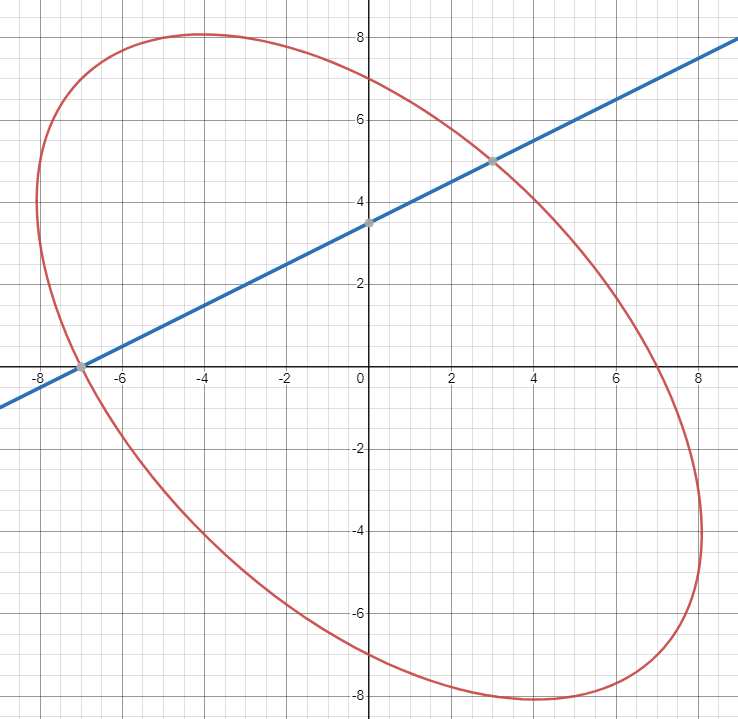
\includegraphics[scale=0.5]{graphing-line-ellipse.png}
\end{center}
\item A line is given by the slope-intercept form
\begin{equation*}
y = -\frac{1}{4}x - 3.
\end{equation*}
\begin{enumerate}
\item Find the slope of the line and the $y$-intercept of the line.
\item Put the equation in standard form and find the $x$-intercept of the line.
\item Find the point on the line with $x$-coordinate $2024$, then put the equation in point-slope form using this point.
\end{enumerate}
\item A line is given by the standard form
\begin{equation*}
3x + y = -4.
\end{equation*}
\begin{enumerate}
\item Find the $x$-intercept and $y$-intercept of the line.
\item Put the equation in slope-intercept form and find the slope of the line.
\item Find the point on the line for which the sum of the coordinates is $10$, then put the equation in point-slope form using this point.
\end{enumerate}
\item A line passes through the point $(-5,2)$ and has slope $1/2$.
\begin{enumerate}
\item Write down an equation for this line in point-slope form.
\item Find the slope-intercept form and the standard form of the line.
\end{enumerate}
\item A line passes through the points $(-3,4)$ and $(-3,-4)$. Find an equation for this line.
\item A line passes through the points $(-3,3)$ and $(0,-4)$.
\begin{enumerate}
\item Find the slope of the line.
\item For each of the two given points, find the point-slope form of the line using that point.
\item Find the slope-intercept form and the standard form of the line.
\end{enumerate}
As a check of your answers, rearranging either of the point-slope equations from part (b) should give you the same slope-intercept form and standard form.
\item A line with equation $y = mx + b$ passes through the points $(5,7)$ and $(8,-1)$. Find $m$ and $b$.
\item Find the point at which the line with equation $2023x + 2022y = 2021$ intersects the line with equation $2024x + 2023y = 2022$.
\item Let $\ell$ be the line with equation $y = -4x - 2$ and let $P = (-4, 2)$. The point $Q$ on line $\ell$ which is closest to $P$ is the point for which $\overline{PQ}\perp\ell$. As such, if $\ell'$ is the line through $P$ perpendicular to line $\ell$, then $Q$ is the intersection of $\ell$ and $\ell'$.
\begin{enumerate}
\item Find the slope of $\ell'$.
\item Find an equation for $\ell'$.
\item Find the coordinates of $Q$.
\end{enumerate}
\end{enumerate}

\subsection{Challenge}

\begin{enumerate}[resume]
\item Let $A = (1,1)$, $B = (5,2)$, and $C = (-4,3)$. In this problem, we will find the coordinates of the point $D$ for which quadrilateral $ABCD$ is a parallelogram.
\begin{enumerate}
\item Find the slopes of lines $AB$ and $BC$.
\item Write down an equation for the line through $C$ parallel to $AB$.
\item Write down an equation for the line through $A$ parallel to $BC$.
\item Since $AB\parallel CD$ and $AD\parallel BC$, point $D$ must be the intersection of the lines you found in parts (b) and (c). Use this to find the coordinates of point $D$.
\end{enumerate}
\end{enumerate}